\chapter{The problem}
\label{chp:problem}
The problem that we solved in this thesis is to provide the \textsc{infn} with a machine learning
capable of, given $15$ harmonics of magnetic field measured on a superconducting magnet:
\begin{enumerate}
	\item Recognize whether the magnet underwent a quench event during operation, we will refer
	      to it as Quench Recognition Problem (\qrp) from now on,
	\item Recognize, if the superconductor quenched, how many coils underwent the quench
	      transition and specifically which coils in the magnet transitioned; we will refer to
	      it as Quench Localization Problem (\qlp) from now on.
\end{enumerate}
A field harmonic is a complex function capable of descibing the contribution of a certain multipolar
field (e.g. the coefficient associated with the dipole is $C_0$, while $C_1$ is the quadrupolar
coefficient) to the entirety of the magnetic field, which is a vectorial and continuous quantity.

This problem, as was already said in previous chapters, is a natural extension of the work of
Samuele Mariotto \cite{mariotto2022}\cite{mariotto2022-generic}, who analyzed the behavior of
a gamma of magnets differing in the number of poles. The original dataset only contained the quench
events recorded for every type of magnet, since the number of events for every other magnet type was
less than the number of quenches recorded for the sole quadrupoles (a total of $177$), we chose to
aim for the creation of a model capable of identifying and locating quench events within a
quadrupolar structure.

As was shown in the theoretical introduction to machine learning (\Cref{chp:ml}) we were aiming to
find models capable of giving a very good explanation of the classification outcomes. Having the
ability of explaining what produced the event can be of great help in the context of magnet design,
quench explanation and instrument calibration (e.g. If a new quench antenna needs to be designed the
researchers know that some magnetic field harmonics can be ignored because they do not influence the
result).

In the following two sections we will explore the structure of the dataset used for the project and
then we will learn about the constraints imposed for reproducibility's sake.

\section{The datasets and their meaning}
The dataset used for the project contained a set of four different measurements, each result of a
previous manipulation done by researcher Mariotto on the original measurements of the magnetic field
harmonics.

\begin{itemize}
	\item \emph{An}: the imaginary part of the magnetic field harmonics, since the measurements
	      done for the original experiments were done in a \emph{skew}
	      configuration\comment{\footnote{Magnets are said to be mounted in skew configuration when the
		      positioning of the magnets is at an angle relative to each other, this improves
		      performance and efficiency}}{Quote someone to make sure that the statement holds for
	      accelerator physics. It's important o be able to understand this question: Why should we mount
	      magnets skewed?} this was the
	      table that supposedly contained more information;
	\item \emph{Bn}: the real part of the magnetic field harmonics;
	\item \emph{Cnmod}: the absolute value of the complex coefficient $C_n$;
	\item \emph{Phi}: the phase of the magnetic field harmonics, since in the original
	      analytical method the conclusions regarding the quenched coil within the maagnet were taken
	      based on this value the naïve hypothesis was that the \qlp solution would strongly depend on
	      this.
\end{itemize}

\section{Model selection and model testing procedures}
Reproducibility is an extremely important property of any experiment, as was said in the chapter
dedicated to a light introduction to machine learning theory (\Cref{chp:ml}), it's an important
first step to set the value of the random number generators.

The next step to enforce reproducibility is by use shared pipelines.

Every dataset used in the project is processed using a common pipeline that builds three different
dataframes that are serialized for later reuse:
\begin{itemize}
	\item The \emph{merged} dataframe contains all of the field harmonics for a certain table
	      (e.g. An) or mix of tables (e.g. An, Bn, Cnmod), berfore serialization the dataframe is
	      normalized using an instance of the StandardScaler class, contained in scikit-learn, trained
	      on the dataframe just created (minus the label columns).
	\item The \emph{safe} dataframe contains a small part of the overall data available to us
	      (29 samples), these samples were kept away until the experiments were considered complete.
	      This dataset allowed us to perform a blind test on the model to see whether it was able to
	      generalize well what it learned.
	\item The \emph{reduced} dataframe contains the rest of the points in the original table,
	      it is the main dataframe used to perform all tests and experiments.
\end{itemize}

When it came to model selection and model testing we chose to perform a Nested Cross Validation
procedure (\ncv). As was said in \Cref{chp:ml} the models used during the project were mostly
supervised, and one of the biggest issues with such models is overfitting. In the following section
we will give a gentle introduction to Cross Validation as a solution to the overfitting problem.

\subsubsection{Cross Validation}
In \Cref{chp:ml} we talked about the simple train-test splitting procedure, now we will introduce an
alternative technique for splitting that gives us a powerful tool to discover and prevent
overfitting.

In general, given a dataset $D$, $k$-fold $\cv$ \cite{ZhouZhi-Hua2021ML} is a technique for splitting a dataset in $k$
different folds $\fold{i}$, the folds are non-overlapping and about the same size, therefore
$\fold{i} \cap \fold{j} = \emptyset \hspace{5pt} \forall i, j \in k$, and the union of all the folds
is the original dataset ($\bigcup_{i \in \{1, \ldots, k\}} \fold{i} = D$).

The logic behind $\cv$ is to prevent biased decision on the human part by introducing a certain
degree of repetition in the experiment. Let us consider a train-test environment, if we used the
procedure introduced in \Cref{chp:ml}, we would do one splitting, one training run on the training
set $T$ and one run of testing on the generalization set $G$; once the test is completed we have the
performance of the model.

\medskip

'What if the split that was chosen was the lucky one and the performance are actually better than
they would be if we took another generalization set?'

\smallskip

This is where $\cv$ comes in, to reduce the probability that the performance of the model
are good just because of a statistical anomaly we increase the number of train-test splits, in fact,
each of the $k$ folds will be used to do testing once, all other folds will be used to do training
on the model.

\medskip

'What value of $k$ should be chosen?'

\smallskip

The number of folds to be used for $\cv$ becomes another hyperparameter of the problem, since it
depends on many factors like the amount of data available to us, a very big value of $k$ will
decrease the size of the testing or generalization fold, which reduces the trust that we can put in
the generalization performance obtained for the model; too small a value of $k$ makes the $\cv$ less
effective from a statistical point of view. There is also an extreme version of the $\cv$ procedure
which is known as Leave One Out (\textsc{loo-cv}), it trains the model on the whole dataset minus
one sample, which is later used for testing, due to the length and complexity this \textsc{loo-cv}
is rarely used in real experiments (despite the high grade of reliability of the results obtained
through it), an efficient version of \textsc{loo-cv} is discussed in \cite{shao2016}.

Until now to explain $\cv$ we have used the simple example of splitting the dataset between train
and test, to introduce Nested $\cv$ ($\ncv$) we will consider the very common case of having to
choose a model and testing its generalization performance.

In the base case a tripartition of the dataset $D$ can work:
\begin{itemize}
	\item \emph{Training set} $T$,
	\item \emph{Validation set} $V$, this set of samples will be used to test the performance of the
	      model found after the training step,
	\item \emph{Generalization set} $G$, after the model is retrained on $T + V$ the performance are
	      tested on $G$ to see if the model is capable of generalizing effectively.
\end{itemize}

\medskip

'How can we guarantee that the model chosen is the best one, or at least is good enough?'

\smallskip

Quite simply, we can't give any guarantees, we might have gotten the worst possible mix of
hyperparameters and still get good performance during the validation and generalization tests due to
statistical anomalies.

\begin{figure}
	\centering
	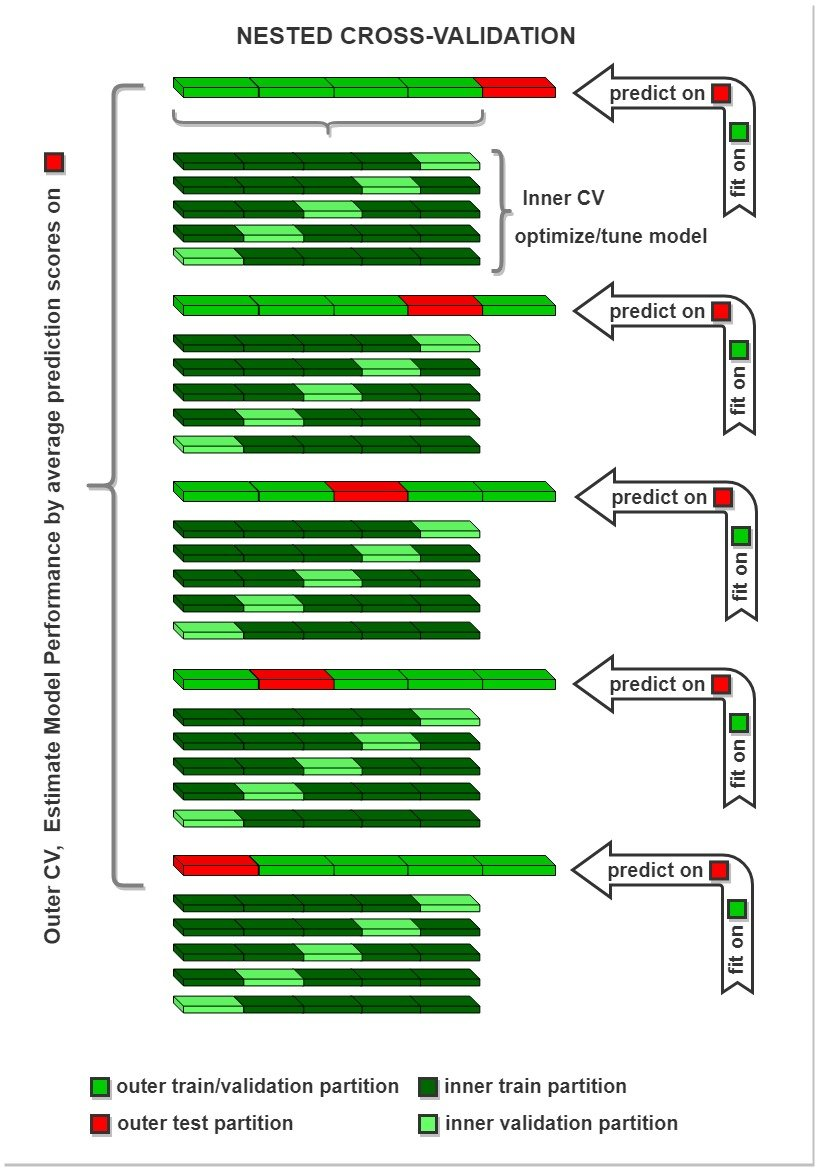
\includegraphics[scale=.3]{./img/nested-cv.png}
	\label{fig:nested-cv}
	\caption{Visualization of the nested cross validation procedure taken from \cite{pain2020}}
\end{figure}
\comment{If I want to add a picture for simple cross validation then something ad hoc should be
created so that the style is kind of the same}

The $\ncv$ is sketched in $\Cref{fig:nested-cv}$, this procedure consists in two simple $\cv$
procedures nested, The outer one is used for testing the generalization performance of the model,
the internal one is used to do model selection and is constructed on the training set used in the
outer loop.

Concretely in the project we chose to apply a $5 \times 5 \ncv$ procedure, which means that, out of
the $250$ samples that form the original dataset $D$:
\begin{itemize}
	\item The data is first split between $50$ samples, that will be kept on the side for the
	      generalization test of the model, and $200$ samples, which will be used to do both
	      training and model selection;
	\item The training set is now split again in $5$ folds, $160$ samples will be used to do
	      model selection (therefore hyperparameter space search), $40$ samples will be used
	      to validate the performance that has been found;
	\item The model found at the previous step is retrained on the whole $200$ samples and then
	      the performance are tested on the fold that was kept aside in the first step.
\end{itemize}
If we consider once again $\Cref{fig:nested-cv}$ it's clear that what comes out of the $\ncv$
procedure are $5$ different models, which one should be considered the best model overall? \comment{We have the guarantee that the models obtained using this procedure are statistically
equivalent}{Citation for this please}.

The scikit-learn library contains many $\cv$ implementations that can give different or stronger
guarantees if compared to the $\cv$ procedure shown in this section, the splitting procedure is also
handled differently based on the type of KFold object used.

The following section used to close this chapter will contain a summarization of the experiment's
characteristics.

\subsection{Experimental setup}
The project was developed using the latest version of the Python programming language
(\texttt{3.10.12} at the moment of writing), a virtual environment was set up to favor ease of use
and the libraries were handled using the pip package manager (also in the last version, which is the
\texttt{24.2}).

Datasets were handled by using a mix of Pandas DataFrames and Numpy N-dimensional arrays. All the
preprocessing and machine learning models used were taken from the scikit-learn library. All the
libraries were used in the latest version available.

The original data consisted of $279$ samples, for \qrp, each sample contained $15$ harmonics and a Label
stating whether the sample represents a quench event or not, for \qlp, each sample had $4$ different
labels associated to it representing whether one of the coils ($0$ for East, then: North, West and
South) quenched or not.

The seeds from the various random number generators have been set to the common value of $42$ to
prevent too much deviation in the experiments.

Dividing the dataset into reduced and safe was completed by using stratified sampling, if
multiclass-classification was required I decided to use the stratified sampling technique provided
in the scikit-multilearn library (\cite{skmlearn}).

As far as the model selection, training and testing pipeline is concerned, as was said in the
previous section, we chose to use a $5\times5 \ncv$ procedure, the model best model was the one
contained in the \_best\_estimator attribute of the GridSearchCV procedure, the resulting
model is then trained on the whole reduced dataset and serialized using pickle.

Experiments were conducted on three different computers running different architectures and
different operating systems, but the results did not change due to the standard-oriented approach,
\Cref{tbl:computers} for a summary of the computers we used.
\begin{center})
	\begin{longtable}{|c|c|c|c|}
		\caption{System information}\label{tbl:computers}
		\\\textbf{}                             & \textbf{Pigna}
		                                                & \textbf{Mattone}
		                                                & \textbf{Topone}
		\\\hline\hline
		\endfirsthead\hline\endlastfoot

		\textbf{CPU manufacturer}                       & Intel
		                                                & AMD
		                                                & Intel
		\\\hline
		\textbf{CPU model}                              & i$5$ $5287\textsc{u}$
		                                                & Ryzen $3700\textsc{x}$
		                                                & i$7$ $4770$
		\\\hline
		\textbf{CPU core count}                         & $2\textsc{c}$ $2\textsc{t}$
		                                                & $8\textsc{c}$ $16\textsc{t}$
		                                                & $4\textsc{c}$ $8\textsc{t}$
		\\\hline
		\textbf{Litography (nm)}                        & $14$
		                                                & $7$
		                                                & $22$
		\\\hline
		\textbf{Launch Date}                            & Q$1$ 2015
		                                                & Q$2$ 2019
		                                                & Q$2$ 2013
		\\\hline
		\textbf{Base frequency (GHz)}                   & $2.90$
		                                                & $4.125$
		                                                & $3.40$
		\\\hline
		\textbf{Boost frequency (GHz)}                  & $3.30$
		                                                & $4.40$
		                                                & $3.90$
		\\\hline
		\textbf{Cache} ($\textsc{mb}$)                  & $3$
		                                                & L1: $0.512$, L2: $4$, L3:$32$
		                                                & $8$
		\\\hline
		\textbf{TDP\footnote{Thermal Design Power} (W)} & 28
		                                                & 84
		                                                & 65
		\\\hline
		\textbf{Memory size} ($\textsc{gb}$)            & $8$
		                                                & $16$
		                                                & $16$
	\end{longtable}
\end{center}








